\documentclass[a4paper,12pt]{report}
\usepackage[utf8]{inputenc}
\usepackage[portuguese]{babel}
\usepackage{graphicx}
\usepackage{hyperref}
\usepackage[utf8]{inputenc}  % Suporte a caracteres UTF-8
\usepackage[T1]{fontenc}     % Codificação de fonte para caracteres especiais
\usepackage[portuguese]{babel}
\usepackage{listings}


% Configurações da Capa
\title{AgroLink - Implementação}
\author{}
\date{Maio 2024}

\begin{document}
	
	% Capa
	\begin{titlepage}
		\centering
		{\scshape\LARGE Coimbra Business School \par}
		\vspace{1cm}
		{\scshape\Large Informática de Gestão - 3º Ano \par}
		\vspace{1.5cm}
		{\huge\bfseries AgroLink - Implementação \par}
		\vspace{2cm}
		
\includegraphics[width=0.3\textwidth]{AGROLINK.png} % Imagem com tamanho definido
		\vspace{3cm}
		\large
		\\Nuno Nogueira (a2021156399)\\
		Paulo Gonçalves (a2020130672)\\
		Tiago Moita (a2021142357)
		\vfill
		Orientador: Professor Paulo Soares \par
		\vfill
		{\large Maio 2024 \par}
	\end{titlepage}
	
	% Resumo
	\newpage
	\chapter*{Resumo}
	 O estudo dedicado ao tema que a seguir se apresenta, AgroLink - Implementação, diz respeito a uma etapa do trabalho que identifica a fase de implementação da aplicação informática AgroLink. Apresentam-se seguidamente alguns constrangimentos que surgiram durante o processo de desenvolvimento da aplicação, bem como os desvios em relação ao especificado na segunda entrega do trabalho anteriormente realizado, assim como as melhorias que se preveem que sejam implementadas. O relatório 	 incluirá uma introdução ao projeto, uma breve descrição das tecnologias utilizadas, uma apresentação da aplicação desenvolvida até ao momento com as suas principais funcionalidades, e uma conclusão com as considerações finais. Toda a documentação de apoio ao trabalho desenvolvido até à presente data, onde se menciona toda a informação relevante, encontra-se disponibilizada na plataforma GitHub  em  \href{https://github.com/nunonogueira03/ProjetoFinal}{ProjetoFinal}.
	 
	% Sumário
	\newpage
	\tableofcontents	
	
	\chapter{App Agrolink}
	A AgroLink foi concebida para otimizar processos e melhorar os rendimentos das explorações de pequenas e médias empresas do setor agrícola, oferecendo soluções práticas e acessíveis que atendem às necessidades específicas dos produtores.
	
	A aplicação surge como resposta às exigências do setor agrícola, que permanece em constante evolução, onde eficiência e produtividade são cruciais para o sucesso. Através deste sistema, os agricultores terão acesso a uma variedade de recursos e funcionalidades projetadas para simplificar tarefas diárias, como gestão de culturas, monitorização de condições climáticas, gestão de tarefas e visualização macro da exploração. Além de promover a eficiência operacional, a AgroLink visa incentivar a
	sustentabilidade e a inovação no setor agrícola, facilitando o acesso a práticas agrículas responsáveis e tecnologias avançadas. O desenvolvimento da AgroLink será guiado pelos seguintes parâmetros:
	
	\begin{itemize}
		\item Facilitar o acompanhamento e a gestão de culturas agrícolas;
		\item Fornecer informações atualizadas sobre as condições climáticas locais;
	     \item Proporcionar uma visão macro das atividades da exploração.
	\end{itemize}
		
	\section{Funcionalidades}
	AgroLink é uma aplicação informática, já referenciada anteriormente em outros documentos, que pretende funcionar como uma plataforma de gestão ao apoio do trabalho das empresas agrícolas. As funcionalidades da plataforma permitem gerir as diferentes frações do terreno ou propriedade. Deste modo, será possível visualizar as tarefas efetuadas em cada uma das frações programadas e obter relatórios, através de sensores localizados no terreno, que em articulação com outra informação obtida, promove a eficácia da gestão, por parte dos seus dos utilizadores.
	
	Mais uma vez se reforça a importância desta plataforma como um recurso fundamental ao desenvolvimento do setor de gestão agrícola. A AgroLink oferece uma interface intuitiva que	permite aos agricultores gerir de forma eficaz as suas operações diárias. 
	
	A aplicação permite a gestão detalhada das diferentes frações do terreno. Os agricultores podem registar e visualizar as frações do terreno, com informações sobre localização e tipo de cultura. Também é possível acompanhar o histórico de atividades realizadas em cada fração com a realização de relatórios e tarefas, uma vez que a aplicação possui uma robusta funcionalidade de relatórios, que permitem aos agricultores a sua análise e tomar decisões mais informadas. Poderá também ser útil no caso do registo e programação das plantações, irrigação, fertilização e colheita, bem como monitorizar o estado atual de cada fração, incluindo as informações obtidas através dos sensores instalados no terreno, como referido
	anteriormente.
	
	A AgroLink facilita a organização e o acompanhamento das tarefas agrícolas, esta permite que os agricultores possam criar tarefas específicas em diferentes frações do terreno, definir prazos e prioridades e receber notificações automáticas sobre as tarefas pendentes ou por concluir. Deste modo as funcionalidades da plataforma possibilitam a criação de relatórios para cada fração do terreno, para que possam ser identificadas as tendências da produção e poder refletir sobre as mesmas e facilitar o planeamento futuro.
	
	A aplicação informática AgroLink desenvolve-se a partir de sensores eletrónicos colocados no terreno, e que permitem fornecer  informação/dados em tempo real. Permite que os agricultores possam monitorizar a unidade do solo, temperatura, níveis de nutrientes e
	outras condições ambientais, dependendo do tipo de sensor que é instalado no solo. A aplicação facilita o envio de alertas automáticos, em condições que sejam detetadas como anómalas ou críticas, permitindo uma rápida atuação para reparação do problema. A aplicação facilita uma gestão eficiente pelos seus utilizadores, garantindo que cada membro da equipa tenha um acesso adequado de acordo com as suas funções no seu posto de trabalho. Os administradores/agricultores podem criar e gerir perfis de utilizador com diferentes níveis de acesso e permissões, atribuir tarefas e monitorizar o desempenho de toda a exploração agrícola, mantendo um histórico de atividades, para garantir a integridade
	e melhoria das funções profissionais e da produtividade. Estas funcionalidades, tornam a AgroLink uma ferramenta essencial, para uma gestão eficiente, em particular de pequenas e médias explorações, promovendo a eficiência, a sustentabilidade e a inovação neste setor Agrícola.
	
	% Capítulo 1
	\chapter{Implementação}
	Na base da criação da aplicação AgroLink, esteve subjacente o recurso a várias plataformas e tecnologias. A sua implementação foi dividida em duas partes	: frontend e backend . O acesso à base de dados e modo como foi desenvolvido o código apresenta-se descrito, através de algumas possibilidades e alternativas, em cada momento do processo, que conduziu à criação desta aplicação informática.

	\section{Base de Dados}
	A base da criação da aplicação AgroLink foi desenhada e implementada no Microsoft SQL Studio, e todas as chamadas de escrita ou leitura são feitas através do backend. Atualmente a
	comunicação é feita através de ficheiros locais JSON. Estes ficheiros JSON são utilizados para transferir os dados entre a aplicação e a base de dados. Quando a aplicação necessita de ler ou
	escrever dados na base de dados, o backend gera um ficheiro JSON com a estrutura e os dados necessários. Este ficheiro é então processado pela aplicação, que realiza a operação correspondente (leitura ou escrita) na base de dados. Este método de comunicação utiliza ficheiros JSON, que permitem uma fácil transferência de dados entre a aplicação e a base de dados, mantendo a integridade e a estrutura dos dados de forma consistente. O objetivo é futuramente fazer-se uma implementação com um servidor externo, de forma a simular um cenário o mais realista possível. A base de dados sofreu algumas alterações devido à inconsistência de alguns dados e por não terem sido ainda implementadas algumas medidas
	de segurança, como é o caso da adição do “sal” nos parâmetros do utilizador. O “sal” é um valor aleatório que é adicionado às passwords antes de lhes ser aplicada a função de hash.
	
	Desta forma, o “sal” aumenta-se a segurança, ao prevenir os ataques de dicionário e rainbow tables, pois mesmo que dois utilizadores tenham a mesma password, os seus hashes serão diferentes devido `a inclusão do ”sal”. Cada utilizador tem um “sal” unico e aleatório que é armazenado na base de dados juntamente com o hash das password.
	\section{Backend}

	Para facilitar a escrita do código e obter uma melhor organização, o backend, seja gráfico ou de funções desenvolveu-se separadamente. Um dos ficheiros do projeto contém todas as funções necessárias para o bom funcionamento da aplicação e estas podem ser divididas nas seguintes categorias:
	
	\begin{itemize}
		 \item Funções de comunicação com a base de dados: Responsáveis por realizar todas as operações de leitura e escrita na base de dados, garantindo que os dados sejam armazenados e recuperados de maneira eficiente e segura.
		
		\item Funções de validação de informação dos formulários da aplicação: Garantem que os dados inseridos pelos utilizadores estejam corretos e completos antes de serem processados ou armazenados. Isso inclui a verificação de formatos de entrada, como endereços de e-mail, bem como a garantia de que todos os campos obrigatórios sejam preenchidos.
		
		\item Formas de evitar a ocorrência de erros durante a utilização da aplicação: Implementam mecanismos de tratamento de erros para lidar com situações inesperadas ou dados inválidos de maneira graciosa, minimizando interrupções no uso da aplicação e melhorando a experiência do utilizador. Isso pode incluir a exibição de mensagens de erro amigáveis e a implementação de medidas preventivas para evitar falhas comuns. 
	\end{itemize}
	
	A parte gráfica do código, que está a ser escrita na linguagem kivy, ao contrário do que foi indicado em documentos anteriores, também está separada, podendo ser considerada como código principal, escrito em python. 
	
	Cada página da aplicação tem um ficheiro em python e um
	ficheiro em kivy e depois existe um ficheiro main em python que faz a ligação entre todos os ficheiros da aplicação. O ficheiro python de cada página, tem toda a parte gráfica como os botões, sliders, imagens, labels, etc. O ficheiro em python das páginas, tem a chamada das funções e a ligação entre o resto da aplicação.
	
	\section{Frontend}
	
	 O frontend é toda a parte gráfica da aplicação. A parte gráfica do código está a ser escrita na linguagem Kivy, ao contrário do que foi indicado em documentos anteriores. O frontend também está separado do resto do código, o que contribui para uma melhor organização e manutenção do projeto. O código principal de cada página, escrito em Python, é responsável pela lógica da aplicação e pela comunicação com o backend.
	
	Cada página da aplicação tem um ficheiro em Python e um ficheiro em Kivy. O ficheiro em Kivy define o layout e os elementos gráficos da página, como botões, sliders, imagens, labels, entre outros. Já o ficheiro Python de cada página contém a lógica necessária para interagir com esses elementos gráficos, bem como as chamadas de funções e a ligação com o resto da aplicação.
	
	Existe um ficheiro principal, main.py, que faz a ligação entre todos os ficheiros da aplicação. Este ficheiro inicializa a aplicação, define as rotas entre as diferentes páginas e garante que todas as partes do frontend e backend trabalham em conjunto de forma precisa.
	
	A escolha de Kivy para o desenvolvimento do frontend traz várias vantagens, tais como:
	
		\begin{itemize}
			\item Multiplataforma: Kivy permite o desenvolvimento de aplicações que podem ser executadas em múltiplas plataformas, incluindo Windows, macOS, Linux, Android e iOS.
			
			\item Suporte a interfaces de usuário ricas: Com Kivy, é possível criar interfaces de usuário modernas e responsivas, que melhoram a experiência do utilizador.
			Comunidade e documentação: Kivy tem uma comunidade ativa e uma boa documentação, o que facilita a resolução de problemas e a aprendizagem de novos conceitos.
		\end{itemize}
	
	Além disso, a separação entre o frontend e o backend permite que os desenvolvedores trabalhem em diferentes partes da aplicação de forma independente, aumentando a eficiência e a produtividade da equipa.
	
		% Capítulo 3
	\chapter{Progressos}
	\section{Desvios}
	Deste os últimos documentos produzidos, foram adicionadas algumas partes e atualizadas
	outras na aplicação AgroLink. A seguinte \ref{fig:BaseDeDados}, apresenta uma base de dados atualizada. Foram adicionadas algumas tabelas, removidas outras e em algumas situações foram implementados novos atributos.
	
		\begin{figure}[!h]
			\centering
			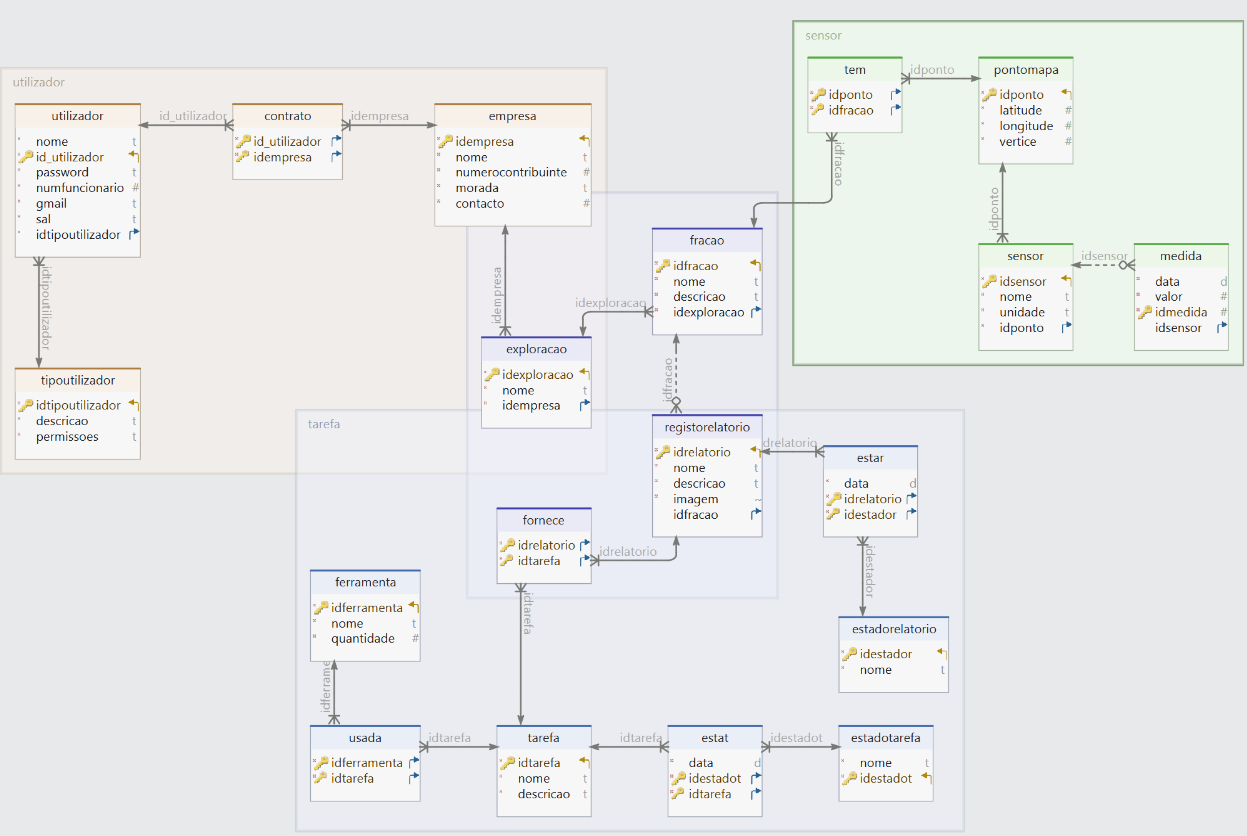
\includegraphics[width=0.7\linewidth]{BaseDeDados.png}
			\caption{Base De Dados}			\label{fig:BaseDeDados}
		\end{figure}

	Numa fase inicial do trabalho toda a comunicação com a base de dados efetuou-se de forma direta através de Querys SQL. Atualmente, essa comunicação é realizada através de ficheiros JSON. Esta mudança foi implementada para assegurar a integridade dos dados e para garantir que, no futuro, não haja problemas na comunicação com o servidor.
	
	A parte gráfica da aplicação foi inicialmente mencionada em versões anteriores como sendo desenvolvida na linguagem Beewave. No entanto, a implementação atual está a ser feita com a linguagem Kivy, devido à disponibilidade de uma documentação mais abrangente e ao suporte de uma comunidade maior e mais ativa. Esta mudança visa garantir um desenvolvimento mais eficiente e a capacidade de resolver problemas de forma mais rápida, aproveitando os recursos e o conhecimento compartilhado pela comunidade Kivy.
	
	Inicialmente, o código foi estruturado para ser dividido em dois tipos de ficheiros principais: funções e o ficheiro principal (main). No entanto, à medida que o desenvolvimento avançava, percebemos que seria muito mais eficiente e organizado dividir o código em várias sub-frações. 	Atualmente, a estrutura do código é composta por:
		
	\begin{itemize}
		\item Um ficheiro principal (main.py), que serve para arrancar a aplicação e chamar todas as páginas.
		
		\item Um ficheiro de funções, que contém todas as funções necessárias para o funcionamento da aplicação.
		
		\item Dois ficheiros por cada página da aplicação:
		\begin{itemize}
			\item Um ficheiro de design com a extensão .kv (linguagem Kivy), que define o layout e os elementos gráficos de cada página.
			
			\item Um ficheiro de lógica com a extensão .py (linguagem Python), que contém a lógica de chamada de funções e a comunicação com outros componentes da aplicação.
		\end{itemize}
	\end{itemize}
	
	Esta organização modular permite uma maior clareza e facilita na manutenção do código, possibilitando que diferentes partes da aplicação sejam desenvolvidas e atualizadas de forma independente. Além disso, essa estrutura modular torna o código mais escalável e preparado para futuras expansões.
	
	
	\section{Dificuldades}
	A realização deste projeto tem sido um desafio em diversos sentidos. As maiores dificuldades que se sentiram ao longo do processo, surgiram na implementação de várias linguagens, tecnologias e na gestão da grande quantidade de código envolvido. Frequentemente precisámos várias horas de pesquisa, tanto para descobrir como para implementar certas funcionalidades, e ainda, para resolver problemas quando o código não funcionava de acordo com o esperado.
	
	Uma das principais dificuldades foi a integração de diferentes tecnologias. A aplicação utiliza Python para a lógica do backend e a linguagem Kivy para o design do frontend, o que exigiu um esforço considerável para garantir que ambas as partes funcionassem harmoniosamente. A necessidade de compreender profundamente cada uma dessas tecnologias, assim como as suas bibliotecas e frameworks associadas, aumentou a complexidade do desenvolvimento. A adicão de alguns pormenores, como é o caso dos ficheiros JSON, também incrementa um pouco a dificuldade.
	
	Além disso, a depuração do código revelou-se um desafio significativo. Muitas vezes, o código não apresentava erros concretos ou mensagens de erro claras, tornando difícil identificar a causa dos problemas.Tivemos de adotar algumas boas práticas de programação para minimizar erros e melhorar a eficiência do processo de desenvolvimento.
	
	Apesar destas dificuldades, a experiência tem sido enriquecedora e tem proporcionado uma grande aprendizagem, uma vez que nunca tínhamos trabalhado com nenhuma destas tecnologias anteriormente a não ser com a base de dados.
	
	
	% Conclusão
	\chapter{Conclusão}
	Consideramos que a aplicação de ferramentas tecnológicas na agricultura são um eixo fundamental para o desenvolvimento deste setor e da sustentabilidade do planeta terra.
	
	Pensar numa ferramenta de trabalho para a eficiência da gestão empresarial, como a aplicação AgroLink – Implementação, foi um grande desafio, que se tornou também uma grande oportunidade, no sentido de acreditarmos que podemos vir a responder às necessidades e expetativas dos gestores das explorações agrícolas. Estamos conscientes que a criação desta plataforma se desenvolveu a partir de uma formação académica, cujo estudo permitiu o contacto com diferentes áreas de conhecimento e orientação científica, que só desde modo nos foi permitido compreender a importância da informação obtida, através de aprendizagens partilhadas. A reflexão sobre a experiência vivida ao longo de todo o processo foi fundamental na avaliação das ações praticadas e nas medidas de ajustamentos realizados, necessários à implementação desta ferramenta de gestão informática, para procurar responder aos objetivos do trabalho que nos propusemos realizar. A orientação e acompanhamento por parte do professor Paulo Soares assim como toda a documentação de apoio, contribuíram para o sucesso das  funcionalidades da aplicação informática desenvolvida.
	
	Conscientes de que os avanços tecnológicos contribuem também para que os agricultores possam operar de forma mais eficiente e eficaz, na medida em que podem poupar tempo e trabalho; gostaríamos de num futuro próximo ter oportunidade de testar esta aplicação em contexto real, junto de uma empresa do setor agrícola, de forma a permitir uma avaliação externa, sobre o seu contributo efetivo, para a monitorização e aumento da produtividade deste setor, aos olhos do seu administrador.

	
\end{document}
